\documentclass[12pt]{article}
\usepackage[margin=0.75in]{geometry}
\geometry{a4paper}
\usepackage[T1]{fontenc} % 
\usepackage[utf8]{inputenc} % 
\usepackage{graphicx} % 
\usepackage{hyperref} % 

\usepackage{subcaption}
\usepackage{lscape}
\usepackage{mathrsfs}
\usepackage{amsfonts}
\usepackage{upgreek}
\usepackage{multirow}
\usepackage{hyperref}
% \usepackage{xcolor}
\usepackage{booktabs}
\usepackage[table,xcdraw]{xcolor}
\usepackage{afterpage}
\usepackage{lipsum}
\usepackage{amsmath}
\usepackage{graphicx}
\usepackage{calligra}
\usepackage[acronym,toc,automake]{glossaries} %%% with acronysm page number

\usepackage{hyphenat}

\usepackage{physics} % Macros supporting the Mathematics of Physics
\usepackage{siunitx} % SI units package
%\sisetup{output-decimal-marker = {,}} % Comma as decimal marker

\newcommand{\iu}{\mathrm{i}\mkern1mu} % Define upright imaginary unit
\newcommand{\diff}{\mathrm{d}\mkern1mu} % Define upright imaginary unit


% Orientação retrato
\usepackage{rotating}

\usepackage{ulem}

\usepackage{subcaption} % Support for sub-captions
%%% PACOTES GRAFICOS
\usepackage{tikz}
\usepackage{import}
\usepackage{pgfplotstable}
\usepackage{pgfplots}
\usetikzlibrary{calc}
\pgfplotsset{compat=1.9}
\usepackage{caption}
\usetikzlibrary{intersections}
\usepgfplotslibrary{fillbetween}
%%%%%%%%%%%%%%%%%%
% ---

% ---
% Pacotes para referencias
% ---
\usepackage[backend=biber,style=abnt,noslsn,doi=false,isbn=false,url=false,uniquename=false,giveninits,repeatfields,maxcitenames=2,maxbibnames=99,backref=true]{biblatex}
\DefineBibliographyStrings{english}{%
	backrefpage = {Cited on p.},%
	backrefpages = {Cited on pp.}%
}
%,uniquelist=false %%% TO FORCE 1 NAME IN ALL THE CITATIONS
\addbibresource{refs_bibtex.bib}
% ---

% List of symbols using the nomenclature package
% \usepackage{nomencl}%   nomenclature generation via makeindex not included in contents
\usepackage[stdsubgroups,intoc]{nomencl} %%% to include in contents
%\usepackage[stdsubgroups]{nomencl}
\usepackage{longtable,tabu}

\makenomenclature

\immediate\write18{%
	makeindex -s nomencl.ist -o \jobname.nls -t \jobname.nlg \jobname.nlo%
}
%\makenomenclature

%\setlength{\nomitemsep}{-\parskip} % Baseline skip between items
%\renewcommand*\nompreamble{\begin{multicols}{2}}
%	\renewcommand*\nompostamble{\end{multicols}}

%\renewcommand{\nomgroup}[1]{\item{\textbf{General Symbols}}}
%\renewcommand{\nomgroup}[1]{%
%	\ifthenelse{\equal{#1}{H}}{\item[\textbf{Greek letters}]}{%
%		\ifthenelse{\equal{#1}{X}}{\item[\textbf{Superscripts}]}{%
%			\ifthenelse{\equal{#1}{Z}}{\item[\textbf{Subscripts}]}{%
%				\ifthenelse{\equal{#1}{G}}{\item[\textbf{General symbols}]}{%
%					\ifthenelse{\equal{#1}{M}}{\item[\textbf{Mathematical operators and conventions}]}{%
%						\ifthenelse{\equal{#1}{P}}{\item[\textbf{Acronyms}]}{}}}}} }}
%%
%%%%%%%%%%%%

\renewcommand{\nomname}{LIST OF SYMBOLS}
%% This code creates the groups
% -----------------------------------------
\usepackage{etoolbox}


%------------------------------------------------------------------
% Titill
%------------------------------------------------------------------
\title{
    \centerline{\includegraphics[width=100mm]{mopt.eps}}
    \vspace{0.5 cm}
    \textit{OpenPulse} - Open source code for numerical modelling of low-frequency acoustically induced vibration in gas pipeline systems \\
    \hspace{1cm} \\
    \large \textbf{Theory Reference A: Acoustics}\\ 
    \small V1.0
}

\author{
    Diego M. Tuozzo, Olavo M. Silva, Lucas V. Q. Kulakauskas, Jacson G. Vargas\\
    \texttt{dmtuozzo@mopt.com.br}
}

\date{9 Mar 2022}


%------------------------------------------------------------------
% 
%------------------------------------------------------------------

\begin{document}
\maketitle 

\section{\texttt{Set Acoustic Element Type}}

In this section, \acrfull{MMs} and damping formulations are presented considering the cases of a stagnant and a moving fluid medium. The complex wavenumber and density expressions for a 1D hard-walled cylindrical waveguide element are presented. 

\subsection{Stagnant fluid medium} 

Consider a hard-walled straight uniform duct element with cross-section area $S_f$ as shown in Fig.~\ref{fig:duct_element}. Gas properties like mean density $\rho_f$ and speed of sound $c_f$ are assumed to be uniform inside the duct. The volume velocity and the pressure at the inlet of the element are denoted as $q_1$ and $p_1$, while $q_2$ and $p_2$ denote the corresponding quantities at the outlet. $Z_f= z_f/S_f = \rho_f c_f / S_f$ represents the acoustic fluid impedance of the duct element (specific impedance $z_f$ divided by the duct element cross-sectional area $S_f$ \cite{kinsler2000fundamentals}).

\begin{figure}[ht!]
	\centering
	%\def\svgwidth{0.4\textwidth}
	%\import{images}{duct_element.pdf_tex}
	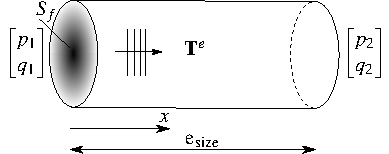
\includegraphics[scale=1.3]{images/0-/duct_element.pdf}
	\caption{Uniform duct element. Figure created by the author.}
	\label{fig:duct_element}
\end{figure}

In a stagnant fluid medium, a \acrfull{MM} is used to represent the wave propagation in a rigid walled cylindrical straight duct element as indicated in Fig.~\label{fig:duct_element}. This elemental matrix is named $\mathbf{K_{\text{A}}}^e$ and is presented in the expanded form with $p, q$ nodal vectors as

\begin{equation} \label{eq:mmm_element_expand}
	\begin{bmatrix}
		- i \, \cot(k_c x)/Z_{f} & i / Z_{f} \sin(k_c x) \\
		i / Z_{f} \sin(k_c x) & -i \, \cot(k_c x) / Z_{f}
	\end{bmatrix}
	\begin{Bmatrix}
		p_1 \\
		p_2
	\end{Bmatrix}
	=
	\begin{Bmatrix}
		q_1 \\
		q_2
	\end{Bmatrix}, 
\end{equation}

\noindent where the definitions of $k_c$ and $Z_f$ will change accordingly with each damping model (Subsections~\ref{subsubsec:proportional}~to~\ref{subsubsec:lrf_damp}), and as a consequence, three different \acrshort{MMs} (apart from the classical undamped wave propagation model) will be generated maintaining the same matrix structure as Eq.~\ref{eq:mmm_element_expand}.

The \acrshort{LRF}-full damping model (Subsection~\ref{subsubsec:lrffull_damp}), has a different \acrshort{MM} because how the viscothermal effect is represented differs from the other three presented models \cite[see][]{TIJDEMAN19751}. The expanded straight tube element matrix $\mathbf{K_{\text{A}}}^e$ with $p, q$ nodal vectors for this damping model is

\begin{equation} \label{eq:mm_system_complete_damped_lrf_full} 
	\frac{i \, S \, \Gamma \, <\beta>_r}{z_0 \, \sinh(\Gamma k_0 \, x)}
	\begin{bmatrix}
		-  \,  \cosh(\Gamma k_0 \, x)  & 1 \\
		1 & - \, \cosh(\Gamma k_0 \, x)
	\end{bmatrix}
	\begin{Bmatrix}
		p_1 \\
		p_2
	\end{Bmatrix}
	=
	\begin{Bmatrix}
		q_1 \\
		q_2 
	\end{Bmatrix}.
\end{equation}

To consider a damped wave propagation, different damping models are used to represent, through the complex wavenumber $k_c$, the viscothermal effect in the acoustic boundary layer. To represent a viscothermal wave propagation, the complex wavenumber is not the unique associated parameter. The complex speed of sound $c_c$ and phase velocity $c_{ph}$ are directly related with $k_c$. These velocities are computed as

\begin{gather} \label{eq:c_c}
	c_c = \frac{\omega}{k_c}, \, \text{and}  \\ \label{eq:c_phase}
	c_{\text{ph}} = \frac{\omega}{\mathcal{R}(k_c)}. %\label{eq:c_phase}
\end{gather}

One of the most frequently used measures of the attenuation capability of a viscothermal damping model for a stagnant fluid is the attenuation coefficient $\alpha_0$. This coefficient is obtained from the negative imaginary part of the complex wavenumber as

\begin{equation} \label{eq:alpha0}
	\alpha_0 = - \mathcal{I}(k_c).
\end{equation}

Other parameters that represent a viscothermal wave propagation are the shear wavenumber $s=r_i \sqrt{\omega / \nu}$ (being $\nu=\mu/\rho_{\text{f}}$ the kinematic viscosity, $\mu$ the dynamic viscosity and $\rho_{\text{f}}$ the fluid density), which physically represents a ratio between inertial and viscous effects and the dimensionless Helmholtz number $He = k r_i$. The inertial effect is represented by the ratio $r_i$ and the viscous effect by the kinematic viscosity $\nu$. Most of the oil and gas pipe engineering applications fulfill the propagation conditions $He<<1$ (plane wave propagation) and $He/s << 1$, generally related with high $s$ values, (i.e. dominant inertial effects, $r_i > \sqrt{\omega / \nu}$, in the acoustic wave propagation and/or plane wave propagation). In addition, varying the pulsation $\omega$ for a fixed fluid and duct radius, inertial or viscous effect can be dominant depending on the $\omega$ value. As defined here, \acrshort{AIV} is not the exception and, in general, $s$ greater than unity is expected for most practical industry applications. Physically, it means that inertial effects start to become dominant rather than viscous effect. 

In engineering applications, sometimes it is useful to relate length scales of an acoustic model. A comparison between the thickness of the viscous or thermal boundary layer ($\delta_v = \sqrt{2 \nu / \omega}$ and $\delta_t = \delta_v / \sqrt{Pr}$ respectively, being $Pr$ the Prandtl number) with a physical dimension of the model (e.g., the tube inner radius $r_i$) is a frequently used length scale, which makes possible to infer the importance of viscous and thermal effects in certain acoustic models. Larger $s$ values can be associated with $\delta_v << r_i$ and $\delta_t << r_i$ (regarding the concept of shear wavenumber previously mentioned).

\subsubsection{Undamped} \label{subsubsec:undamped}

The classical undamped model considers a purely real wavenumber and density, i.e.,

\begin{gather} 
	k_{\text{c}} = k_0 = \frac{\omega}{c_0},  \\
	\rho_{\text{c}} = \rho_0	
\end{gather}

\noindent where $k_0$, $c_0$ and $\rho_0$ are the undisturbed wavenumber, velocity and density of the fluid medium.

\subsubsection{Proportional} \label{subsubsec:proportional}

The classical proportional damping model can be basically interpreted as a viscous-attenuation fluid property. Its value is typically obtained from experimental data and can be expressed as a part of the real value of the complex wavenumber $k_c$. Also, the proportional attenuation coefficient (referred to as the loss coefficient of the material) $\eta$ could be frequency-dependent, $\eta(f)$, or frequency-independent, $\eta$. For a rightward propagating plane wave (omitting time dependence) considering proportional damping, a complex wavenumber can be assumed as

\begin{equation} \label{eq:complex_wavenumber_hysteretic} 
	k_c = k_1 + i k_2 = k_0(1 -i\eta),
\end{equation}

\noindent where $\eta$ is dimensionless. The proportional complex density can be computed as

\begin{equation} \label{eq:complex_density}
	\rho_{c} = \rho_{0} (1-i \eta)^2.
\end{equation}

\noindent The proportional damping model has no limitations on its application related with the $He$ or the $s$ for \acrshort{AIV} problems.

\subsubsection{Wide-duct} \label{subsubsec:wide-duct}

The Helmholtz-Kirchhoff wall-attenuation coefficient, also known as a wide-duct wall attenuation model \cite{temkin1981elements}, is intended to account separately viscous and thermal effects, which are then summed to obtain a total wall-attenuation in tubes with radius $r_i$ relatively large and $\omega$ relatively small. Under the assumption of small dissipation condition and plane-wave propagation (i.e.,  $r < \lambda$, see \cite{temkin1981elements} for more theoretical details), the Helmholtz-Kirchhoff (total) wall-attenuation coefficient can be included in the complex wavenumber as

\begin{equation} \label{eq:complex_wavenumber_wideduct}
	k_c = k_0 - i\frac{\sqrt{\omega \nu_{\text{f}}} }{\sqrt{2}c_{0} r_{\text{i}}} \big( 1 + \frac{\gamma-1}{\sqrt{Pr}} \big),
\end{equation}

\noindent where $Pr$ is the Prandtl number, $\nu_{\text{f}}$ is the undisturbed fluid kinematic viscosity, and $\gamma = C_p/C_v$ the ratio of specific heats. Then, the complex fluid density for the Helmholtz-Kirchoff damping is defined as

\begin{equation}
	\rho_{c} = \rho_{0} \Big[ 1 - i \frac{ \sqrt{ \nu_{\text{f}} } }{ \sqrt{2 \omega } \, c_{0} \,  r_{\text{i}} } \Big( 1 + \frac{\gamma-1}{\sqrt{Pr}} \Big) \Big]^{-2}.
\end{equation}

\noindent The Helmholtz-Kirchoff damping may be accurate within the following assumptions \cite{temkin1981elements}

\begin{gather}
	r_{\text{i}} >> \sqrt{\frac{ 2 \nu_{\text{f}} }{\omega}}, \\
	r_{\text{i}} >> \sqrt{\frac{ 2 \kappa_{\text{f}} }{\omega}}, \\
	\frac{\omega \nu_{\text{f}} }{ c_{\text{f}}^2 } << 0.5,	
\end{gather}

\noindent where $\kappa_{\text{f}}$ is the undisturbed fluid thermal conductivity, $c_{\text{f}}$ is the undisturbed sound speed of the fluid  and the symbol $<<$ may be interpreted as ``at least one magnitude order of difference''.

\subsubsection{LRF fluid equivalent} \label{subsubsec:lrf_damp}

The \acrfull{LRF} model (named by Tijdeman \cite{TIJDEMAN19751}) describes viscothermal acoustics in uniform tubes and layers that have a cross-section smaller than the acoustic wavelength (inside the plane wave frequency range). Inside the low-frequency range, this model covers from very narrow tubes to large ducts where the boundary layer only represents a fraction of the duct size (wide tubes).

The approximate viscothermal solution obtained from solving the Eqs.~3.10a~and~3.10b in Chapter~3 in \cite{kampinga_phdthesis} derive into the solutions for the velocity, temperature and density \cite[Eqs.~3.27 in Chapter~3 in][]{kampinga_phdthesis}. The Eq.~3.28 in Chapter 3 in \cite{kampinga_phdthesis} will allow us to calculate the \acrfull{LRF-EF} complex wavenumber $k_c$ for cylindrical waveguides. With $k_c$, the viscothermal effect can be introduced onto the fluid. In \textit{OpenPulse}, the \acrshort{LRF-EF} complex wavenumber $k_c$ is implemented as

\begin{equation} \label{eq:complex_wavenumber_lrf_ef}
	k_c= k_0 \, \sqrt{\frac{\Upsilon_t'}{\Upsilon_v} }, 
\end{equation}

\noindent where $\Upsilon_t'=\gamma - (\gamma - 1) \Upsilon_t$ is the modified cross-sectional mean thermal field, in which $\Upsilon_t$ (the cross-sectional mean thermal field) and also $\Upsilon_v$ (the cross-sectional mean viscous field) are defined, for cylindrical waveguides, as

%\begin{align}
%	& \Upsilon_t = \big< \Psi_t\big>_{\partial \Omega} = \frac{1}{S}\int_{\partial \Omega}  \Psi_t \diff \partial \Omega = \frac{1}{S}\int_{0}^{r_\text{i}}  1 - \frac{J_0 (k_t r)}{J_0 (k_t r_\text{i})} \diff r=  -\frac{J_2(k_t r_\text{i})}{J_0(k_t r_\text{i})}, \\
%	& \Upsilon_v = \big< \Psi_v\big>_{\partial \Omega} = \frac{1}{S}\int_{\partial \Omega}  \Psi_v \diff \partial \Omega = \frac{1}{S}\int_{0}^{r_\text{i}}  1 - \frac{J_0 (k_v r_\text{i})}{J_0 (k_v r_\text{i})} \diff r= -\frac{J_2(k_v r_\text{i})}{J_0(k_v r_\text{i})},
%\end{align}

\begin{align}
	& \Upsilon_t =  -\frac{J_2(k_t r_\text{i})}{J_0(k_t r_\text{i})}, \\
	& \Upsilon_v = -\frac{J_2(k_v r_\text{i})}{J_0(k_v r_\text{i})},
\end{align}

\noindent where $J_0$ and  $J_2$ are the Bessel function of the first kind and zeroth and second order, respectively, and $k_v = \sqrt{ -i \omega \rho_0 / \mu } $ and $k_t = \sqrt{ - i \omega \rho_0 C_p / \kappa}$ the viscous and thermal wavenumber, respectively \cite{kampinga_phdthesis}.

\noindent Considering an harmonically varying pressure $p$, the Eq.~\ref{eq:complex_wavenumber_lrf_ef} and defining the axial velocity, accordingly to the \acrshort{LRF} model presented in the work of Kampinga \cite[Eq.~3.46a in][]{kampinga_phdthesis}, on the form

\begin{equation} \label{eq:velocity_lrf}
	u(x) = \frac{i \Upsilon_v \nabla p}{k_0 z_0}, 
\end{equation}

\noindent the complex fluid impedance can be calculated using the impedance definition only retaining the rightward propagating pressure term (freely propagating plane wave)

\begin{equation} \label{eq:zc_lrfef}
	z_c = \frac{p(x,t)}{u(x,t)} = \frac{z_0}{\sqrt{\Upsilon_v \Upsilon_t'}}.
\end{equation}

\noindent With Eqs.~\ref{eq:complex_wavenumber_lrf_ef}~and~\ref{eq:zc_lrfef}, the complex fluid density can be defined as

\begin{equation}
	\rho_{c} = \frac{ z_c k_c }{ \omega  } =\frac{ \rho_{0} }{ \Upsilon_v  }.
\end{equation}

\noindent The \acrshort{LRF-EF} damping model may be accurate within the following assumptions \cite{kampinga_phdthesis} 

\begin{gather}
	\frac{ k_{\text{t}} }{ k } >> 1, \\
	\frac{ k_{\text{v}} }{ k } >> 1.	
\end{gather}

Details about the \acrshort{LRF-EF} model and expressions for the mean thermal and viscous field ($\Upsilon_t$ and $\Upsilon_v$) as well as the viscous and thermal wavenumbers .($k_v$ and $k_t$) for different fluid cross-section geometries can be found in \cite[pp.62 and 63 and Appendix A in][]{kampinga_phdthesis} and also related papers.

%Then, the Eq.~3.28 in \cite{kampinga_phdthesis} is reproduced as
%
%\begin{equation} 
%	\nabla \cdot \mathbf{v} + i \frac{k_0}{z_0} \Psi'_{\text{t}} p = 0,
%\end{equation}
%
%\noindent where $\Psi'_{\text{t}} = \gamma - (\gamma - 1)\Psi_{\text{t}}$ is the modified thermal field, $\Psi_{\text{t}} = 1 - ( J_0 (k_t r)/ J_0 (k_t l))$ is the thermal field (for cylindrical waveguides) and $\mathbf{v}$ is the velocity field \cite[Eq.~3.27 in][]{kampinga_phdthesis} . $p$ is defined as a harmonic pressure variation on the form
%
%\begin{equation} \label{eq:pressure_lrf}
%	% \begin{gather} 
%		p(x) =  (A e^{-i k_c x} + B e^{ i k_c x}) e^{i\omega t}.
%		% u(x) = \frac{i \upsilon_v \nabla p}{k_0 z_0} 
%		% \end{gather}
%\end{equation}
%
%\noindent Then, it is possible to calculate the \acrshort{LRF-EF} complex wavenumber $k_c$ as

\subsubsection{LRF full} \label{subsubsec:lrffull_damp}

In this subsection, another \acrshort{LRF} model is presented, but not using the complex wavenumber as a way to introduce the viscothermal effects onto the bulk. The \acrshort{LRF}-full model presented here uses the pressure, temperature, axial velocity and density field solutions from the \acrshort{LRF} approximation for cylindrical waveguides. The denomination $full$ is related to the fact that the pressure and the axial velocity \acrshort{LRF} solution obtained by Tijdeman \cite{TIJDEMAN19751} were used to build the \acrshort{MM} presented in  Eq.~\ref{eq:mm_system_complete_damped_lrf_full}.

The model is obtained assuming no-slip and isothermal \acrshort{BC's} at the wall of the tube and also an axial symmetric velocity profile as \acrshort{BC}, and imposing a harmonic pressure perturbation as

\begin{equation} \label{eq:pressure_lrf_full}
	p(x,t) = \frac{\rho_0 c_0^2  }{\gamma} ( A e^{\Gamma k_0 x } + B e^{- \Gamma k_0 x} ) e^{i \omega t},
\end{equation}

\noindent where the following dimensionless numbers are the base of this model:

\begin{gather}
	\Gamma = \sqrt{ J_0(i^{3/2} s)   / J_2(i^{3/2} s) } \sqrt{  \gamma / n }, \\
	s = r_i \sqrt{\omega / \nu}, \\
	\gamma_p = \Big[ 1 + ((\gamma-1)/\gamma) ( J_2(i^{3/2} \sigma s)   / J_0(i^{3/2} \sigma s)  )\Big]^{-1}, \\
	\sigma = \sqrt{\mu C_p / \kappa} = \sqrt{Pr},
\end{gather}

\noindent where $\Gamma$ is the propagation constant, $s$ is the shear wave number (also referred as the Stokes number), $\gamma_p$ is the politropic constant and $\sigma$ is the square root of the Prandtl number. Consequently, the solution for the axial velocity is (omitting time dependence)

% \begin{equation} \label{eq:velocity_lrf_full}
	%     u = \frac{i c_0 \Gamma}{\gamma} \Big[ 1 - \frac{ J_0( i^{3/2} \eta s ) }{J_0( i^{3/2} s ) } \Big] ( A e^{\Gamma k x } - B e^{- \Gamma k x} ),
	% \end{equation}
\begin{equation} \label{eq:velocity_lrf_full}
	u(x) = \frac{i c_0 \Gamma}{\gamma} \beta ( A e^{\Gamma k_0 x } - B e^{- \Gamma k_0 x} ).
\end{equation}

% being $\eta = r/r_i$ a dimensionless radial coordinate for the moving parameter $r$ and the fixed value of the inner tube radius $r_i$ ($R$ in Tijdeman's notation).

\noindent where $\beta = 1 - \big( J_0(i^{3/2} \zeta s) /J_0(i^{3/2} s) \big)$, in which $J_0$ is the Bessel function of the first kind and zeroth order,  $\zeta = r/r_i$ is a dimensionless radial coordinate for the moving parameter $r$ and the fixed value of the inner tube radius $r_i$ ($\eta = r/R$ in Tijdeman's notation). 

As can be seen, the Eqs.~\ref{eq:pressure_lrf_full}~and~\ref{eq:velocity_lrf_full} are radial and axial dependent. Both \acrshort{TMM} and \acrshort{MMM} are based on 1D \acrshort{TM} and \acrshort{MM}. In this case, Eqs.~\ref{eq:pressure_lrf_full} and \ref{eq:velocity_lrf_full} need to be integrated over the cross-section to obtain the 1D \acrshort{TM} and \acrshort{MM} (Eqs.~\ref{eq:TMM_system_complete_LRF_full}~and~\ref{eq:mm_system_complete_damped_lrf_full}, respectively). This integration is based on the parameter $\beta$ and is executed as indicated in Eq.~\ref{eq:alpha_avrg}. For more theoretical details, the reader is invited to consult \cite{TIJDEMAN19751, stinson}.

The propagation constant $\Gamma = \mathcal{R}(\Gamma) + i \, \mathcal{I}(\Gamma)$ is one of the dimensionless parameters used in \cite{TIJDEMAN19751} to describe a wave motion considering inertia, compressibility, viscosity,
and thermal conductivity of a fluid in a cylindrical tube in \cite{TIJDEMAN19751}. The relation between $\Gamma$ and $k_c$ is presented as \cite{TIJDEMAN19751,eerden_phdthesis_2000,mareze_jsv}

\begin{equation}\label{eq:kc_lrffull}
	k_c = -i \Gamma k_0.
\end{equation}

\noindent Moreover, the complex density is calculated utilizing Eq.~\ref{eq:complex_density}. Consequently,

\begin{equation}
	\rho_c = \frac{z_c k_c}{\omega} = \frac{\rho_0}{<\beta>_r},
	%    \frac{ \rho_0  }{ <\beta>_r  }.
\end{equation}

\noindent where $z_c = i z_0 / (\Gamma <\beta>_r)$ is the medium-specific impedance of a propagating plane wave when duct viscothermal effect is included and $<\beta>_r$ is the average of $\beta$ over the tube cross section, defined as

\begin{equation} \label{eq:alpha_avrg}
	<\beta>_r = \frac{1}{S_f} \int_{r} 2\pi r \beta(r) \text{d}r = 1 - \frac{2 J_1 \big( s \sigma (\sqrt{2}/2) (1 - i) \big) }{  (s \sigma (\sqrt{2}/2)  (1 - i) ) J_0 \big( s \sigma i^{3/2} \big)   }.
\end{equation}

%and the complex speed of sound can be expressed as
%
%\begin{equation}
%    c_c = \frac{i c_0}{\Gamma}.
%\end{equation}

\noindent The LRF-full damping model may be accurate for the following shear wave number condition \cite{TIJDEMAN19751} 

\begin{equation}
	s \geq 4, \\	
\end{equation}

\noindent without limitations inside the plane wave frequency range ($He= k r_{\text{i}} < 1.84118$). However, when $ 1 < s < 4 $ the following limitations related with the Helmholtz number, $He$, may be considered \cite[see Figs.~9~and~10 in][]{TIJDEMAN19751}

\begin{gather}
	He << 1, \\
	\frac{He}{s} << 1.	
\end{gather}


\subsection{Moving fluid medium}

In a moving fluid medium, a \acrfull{MM} is also used to represent the wave propagation in a rigid walled cylindrical straight duct element. The elemental matrix $\mathbf{K_{\text{A}}}^e$, based on the \acrfull{TM} proposed by \cite{TO_meanflow} for an incompressible fluid flow, is presented in the expanded form as

\begin{equation} \label{eq:MM_flow-acoustic}
	\resizebox{0.9\textwidth}{!}{
		$	(Z_f (1 - M'^2) \sinh(i k_c x) )^{-1}
		\begin{bmatrix}
			% (1 /  tanh(i k_c x)) - M' &  - e^{i k_c x} / sinh(i k_c x)  \\
			% - e^{- i k_c x}/ sinh(i k_c x) & (1 / tanh(i k_c x)) + M'
			\cosh(i k_c x) - M' \sinh(i k_c x) &  - e^{-i k_c M' x}  \\
			- e^{i k_c M' x} & \cosh(i k_c x) + M' \sinh(i k_c x)
		\end{bmatrix}
		\begin{Bmatrix}
			p_1 \\
			p_2
		\end{Bmatrix}
		=
		\begin{Bmatrix}
			q_1 \\
			q_2 
		\end{Bmatrix}.$
	}
\end{equation}

\noindent where $k_c$ is the complex averaged wavenumber of a moving fluid medium taking into account the sound-turbulence interaction mechanism through $k_c = (k_+ + k_-) / 2$ in which $k_+$ and $k_-$ are the rightward and leftward wave attenuation coefficients, respectively. The dimensionless Mach number (with damping effects included) is defined as $M'=U/c_c$, in which $c_c = \omega / k_c$ is the complex speed of sound and $Z_f = \rho_0 c_c / S $ is the complex acoustic impedance taking into account the damping effects. The term $Z_f (1 - M'^2)$ in Eq.~\ref{eq:MM_flow-acoustic} represents the acoustic impedance of the moving fluid medium of section $S_f$.

In a moving fluid medium, the damping models of Howe \cite{howe_1995} and Peters \cite{ peters_thesis, peters_hirschberg_reijnen_wijnands_1993} take into account the viscothermal effect in the acoustic boundary layer, the mean flow convection and the turbulent absorption. These effects are dominant in the low $M$ range ($M \leq$ 0.1) and plane wave frequency range ($He(1-M^2) <$ 1.81). These parameters are considered the limit of application in \textit{OpenPulse} of the theoretical background for moving fluid medium. The undamped model only takes into account the mean flow convection.

Apart from the complex wavenumber $k_c$ and the convective Helmholtz number $He(1-M^2)$, other parameters characterize the wave propagation in a moving fluid medium. A pair of these are the dimensionless acoustic boundary layer $\delta_a^+$ and the turbulent viscous sub-layer $\delta_{\nu s}$, both defined by

\begin{gather} \label{eq:ac_bl_dimnesionless}
\delta_a^+ = \delta_a u_{\tau}/ \nu, \\ \label{eq:visc_sublayer}
\delta_{\nu s} \approx 6.5 \nu / u_{\tau},
\end{gather}

\noindent where $\delta_a = l_{vor} = \delta_v = \sqrt{2 \nu / \omega}$ is the dimensional acoustic boundary layer and $u_{\tau}$ is the friction velocity. Here, $\delta_a = l_{vor} = \delta_v$ since in air $Pr$ is close to unity, then, the viscous boundary layer length scale $l_{vor} $ approaches to the thermal boundary layer length scale $l_{ent}= \sqrt{2 \nu / (\omega Pr)}$ \cite{weng_thesis}. The value 6.5 in Eq.~\ref{eq:visc_sublayer} is taken from \cite{howe_1995}, which was obtained using low frequency experimental data fitting. Others authors indicate different values as 5 in \cite{ weng_thesis,tiikoja_2016}, 15 in \cite{ronneberger_ahrens_1977} by experimental fitting and 10 (approximate value) and 12.5 (by experimental data fitting) in \cite{peters_hirschberg_reijnen_wijnands_1993, peters_thesis}. 

The upstream and downstream wave attenuation coefficient $\alpha_{\pm}$, is another parameter used to characterize the attenuation capability of a damping model considering moving fluid medium. It is defined as

\begin{equation}
	\alpha_{\pm} = - \mathcal{I}(\pm k_{\pm}).
\end{equation}

In addition, an averaged attenuation coefficient  $\overline{\alpha}$ can be calculated as in \cite{ronneberger_ahrens_1977, weng_paper3_2015}:

\begin{equation} \label{eq:mean_attenuation}
	\overline{\alpha} = \frac{\alpha_+ + \alpha_-}{2}.
\end{equation}

\subsubsection{Undamped}

If damping effects on the medium are neglected and only mean flow convection is represented, the complex wavenumber $k_c$ is given by 

\begin{equation}
k_c = k = \frac{k_0}{(1-M^2)}.
\end{equation}

\subsubsection{Howe model}

The expressions derived by Howe \cite{howe_1995} for the upstream and downstream wave attenuation coefficient for fully developed turbulent flow $\alpha_{\pm}$, the friction velocity $u_{\tau}$ (empirical formula) and the frequency dependent viscous sub-layer (empirical formula), $\delta_{\text{vs}}$, are presented here since they will be used in the \acrshort{TMs} and \acrshort{MMs} calculations in the following subsection:

%\alpha_{\pm, Howe} = - \mathcal{I}(\pm k_{\pm, Howe}) = - \mathcal{I} \Bigg( \pm \frac{\pm 1 }{ (1 \pm M)} \Bigg\{ k_0 +  \underbrace{ \frac{2 e^{-i \pi /4} \sqrt{\omega \nu} }{c_0 D_p }  \text{Conj} \Bigg[ \frac{ F_{A,1}  }{(1 \pm M)^2}  + \frac{ (\gamma - 1) \sqrt{\chi}  }{ \sqrt{\nu} } F_{A,2} \Bigg] }_\text{wall shear layer correction} \Bigg\} \Bigg), \\
%\vspace{-11mm}

\begin{gather} \label{eq:damping_coeff_howe}
	\alpha_{\pm, Howe} = - \mathcal{I}(\pm k_{\pm, Howe}), \\
	k_{\pm, Howe} = \frac{\pm 1 }{ (1 \pm M)} \Bigg( k_0 +  \underbrace{ \frac{2 e^{-i \pi /4} \sqrt{\omega \nu} }{c_0 D_p }  \Bigg( \frac{ F_{A,1}  }{(1 \pm M)^2}  + \frac{ (\gamma - 1) \sqrt{\chi}  }{ \sqrt{\nu} } F_{A,2} \Bigg)^{*} }_\text{wall shear layer correction} \Bigg), \\
	F_{A,j}=\frac{i ( H_1^{(1)}(a_j) \cos(b_j) -  H_0^{(1)}(a_j) \sin(b_j)) }{ H_0^{(1)}(a_j) \cos(b_j) +  H_1^{(1)}(a_j) \sin(b_j) }, \\ 
	a_1 = \frac{\sqrt{i \omega \nu } }{ \kappa_k u_{\tau}}, \hspace{2mm} b_1 = \delta_{\text{vs}} \sqrt{\frac{i \omega}{\nu}}, \hspace{2mm} a_2 = \frac{\sqrt{i \omega \chi} Pr_t}{\kappa_k u_{\tau}}, \hspace{2mm} b_2 = \delta_{\text{vs}} \sqrt{\frac{i \omega}{\chi}}, \\ \label{eq:shear_velocity_howe}
	\frac{U}{u_{\tau}} = 2.44 \, ln(u_{\tau} D_p / (2 \nu) ) + 2, \\ 
	\frac{\delta_{\text{vs}} u_{\tau}}{\nu} = 6.5 \Big( 1 + \frac{1.7 (\omega / \omega_{*})^3}{1 + (\omega / \omega_{*})^3} \Big) , \hspace{5mm} \omega_{*} \nu / u_{\tau}^2 \approx 0.01 , \hspace{5mm} \omega > 0,  
\end{gather}

\noindent where $(\cdot)^{*}$ indicates complex conjugate of the quantity between parenthesis; $D_p = 4S_f / (\pi d_i)$ is the inner duct's hydraulic diameter; $\kappa_k \approx 0.41$ is the von Karman constant; $Pr_t $ is the turbulent Prandtl number and its value is approximately $Pr_t =0.87$ for flow with $Pr > 0.5 $ \cite{schlichting2016boundary}; $\chi = \kappa/\rho_0 C_p$ is the fluid thermal diffusivity in m$^2$/s, in which $\kappa$ is the thermal conductivity; $F_{A,j}$ is an auxiliary function in which $j=1,2$; $H_0^{(1)}$ and $H_1^{(1)}$ are the Hankel functions of the zeroth and the first order respectively and $a_j$ and $b_j$ are arguments of the auxiliary function $F_{A,j}$. $\omega_{*}$ is defined by Howe \cite{howe_1995} as a critical  frequency. Eq.~\ref{eq:damping_coeff_howe} was validated by Howe using experimental data obtained by Peters et al. \cite[see Fig.9. in ][]{peters_hirschberg_reijnen_wijnands_1993} up to $M = 0.1$. A suggested $Re=\rho r_i U / (2 \mu) > 10^4$ value for justifying some experimental-theoretical differences is based on the high Reynolds number eddy viscosity model adopted in the semi-empirical model of Howe.

\subsubsection{Peters model}

The expressions for the damping coefficient considering the zero Mach number limit $\lim_{M \xrightarrow{}0} \alpha_{\pm}$ and the shear velocity corresponding to the model of Peters et al. are reproduced here from Durrieu et al. \cite{durrieu_2001} as \footnote{There is a mismatch between \cite[Eqs.~(4.1.46)~-~(4.1.48) in][]{weng_thesis} with \cite[Eqs.~(A1)~-~(A6) in][]{durrieu_2001}. To the author knowledge some notation mistake appears to be made in \cite[Eq.~(A5) in][]{durrieu_2001} using $\delta_a$ and  $\delta_l$ instead of $\delta_a^+$ and  $\delta_l^+$, respectively. Another one seemed to be made with the exponential quadratic term in the same equation. Here, the aforementioned Eq.~(A5) was replaced by the original expression defined in \cite[Eqs.~(4.1.47)~and~(17) respectively in][]{weng_thesis,peters_hirschberg_reijnen_wijnands_1993}. It is important to note that the defined damping in stagnant fluid $\alpha_0$ in \cite{durrieu_2001} is not the same that was defined in \cite{weng_thesis, peters_hirschberg_reijnen_wijnands_1993, peters_thesis}.}

%  \lim_{M \xrightarrow{}0} \,
\begin{gather} \label{eq:damping_coeff_peters}
	\alpha_{\pm, Peters} = - \mathcal{I}(\pm \, k_{\pm, Peters}), \\
	k_{\pm, Peters} = \frac{ \pm k_0 }{ (1 \pm M) }  \pm \underbrace{ (1- i)\lim_{M \xrightarrow{}0} \alpha_{\pm, Peters}}_\text{wall shear layer correction},  \\ 
	\lim_{M \xrightarrow{}0} \alpha_{\pm, Peters}  = k_0 \frac{ \delta_{a} }{ d_i (1 \pm M) } \frac{ 1 + e^{-2(1+ i)(\delta_{\text{vs}}^+ /\delta_{a}^+ ) - (200i /\delta_{a}^{+2} )} }{ 1 - e^{-2(1+ i)(\delta_{\text{vs}}^+ /\delta_{a}^+ )} } \Big( 1 + \frac{\gamma -1}{\sqrt{Pr}} \Big), \\ \label{eq:damping_coeff_peters_lowlimit}
	u_{\tau}^2 = \frac{\tau_{\text{w}}}{\rho_{\text{f}}} = 0.03955 \Big( \frac{\nu}{d_i} \Big)^{1/4} U^{7/4},    
\end{gather}

% \begin{equation}
	%     \alpha_{\pm, Peters}  = k_0 \frac{ \delta_{a} }{ d_i (1 \pm M) } \frac{ 1 + e^{-2(1+ i)(\delta_l /\delta_{a} ) - 200i (\delta_l /\delta_{a} )^{2} } }{ 1 - e^{-2(1+ i)(\delta_l /\delta_{a}) } } \Big( 1 + \frac{\gamma -1}{\sqrt{Pr}} \Big)
	% \end{equation}

% where  $\delta_a$ is the dimensional acoustic layer as was previously defined and $\delta_l^+$ is the adimensional viscous sublayer of the turbulent main flow and was determinated by Peters \cite{peters_hirschberg_reijnen_wijnands_1993} as $\delta_l^+ = 12.5$ and  $\delta_{a}^+ = \delta_{a} u_{\tau}/\nu$ in which $u_{\tau}$ is the friction velocity of the mean flow. 

\noindent where $\tau_{\text{w}}$ is the wall shear stress and $\delta_{\text{vs}}^+$ is the dimensionless viscous sub-layer of the turbulent main flow defined by Peters et al. \cite{peters_hirschberg_reijnen_wijnands_1993, peters_thesis} as $\delta_{\text{vs}} = 12.5 \nu / u_{\tau}$, in which 12.5 is a factor obtained by fitting low-frequency quasi-steady limit with experimental data in \cite{ronneberger_ahrens_1977, peters_hirschberg_reijnen_wijnands_1993, peters_thesis}.

\section{\texttt{Set Acoustic Pressure}}

An acoustic pressure is one of the \acrfull{BC's} that can be applied in the \acrfull{FETM} formulation. The prescribed pressure $p_i$ in the global column vector of unknown pressures can be frequency dependent $p_i(\omega)$. The classical process applied in \acrshort{FEM} for prescribed displacement needs to be done as in \cite{eerden_phdthesis_2000,hughes}.

A cross junction model with four duct elements with straight constant section is presented in Fig.~\ref{fig:one_dim_ducts} as an example to show how the \acrshort{FEM}-based \acrshort{BC's} insertion process works.

\begin{figure}[h!]
	\centering
	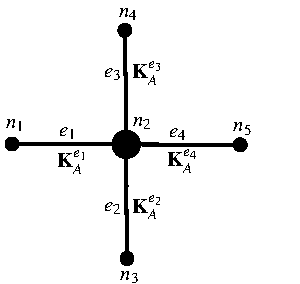
\includegraphics[scale=1.5]{images/0-/one_dim_four_duct.pdf}
	\caption{A 1D cross-junction \acrshort{MM} model with arbitrary node and element indexing.}
	\label{fig:one_dim_ducts}
\end{figure}

The global mobility matrix \acrshort{GMM} of the system in Fig.~\ref{fig:one_dim_ducts} is presented as follows

\begin{equation} \label{eq:assembly_global_mobility_matrix}
	\begin{bmatrix}
		\textcolor{red}{\mathbf{K}_{A}^{e_1}(1,1)} & \textcolor{red}{\mathbf{K}_{A}^{e_1}(1,2)} & 0 & 0 & 0 \\
		\textcolor{red}{\mathbf{K}_{A}^{e_1}(2,1)}  & C & \textcolor{blue}{\mathbf{K}_{A}^{e_2}(1,2)} & \textcolor{green}{\mathbf{K}_{A}^{e_3}(1,2)} & \textcolor{cyan}{\mathbf{K}_{A}^{e_4}(1,2)} \\
		0   &   \textcolor{blue}{\mathbf{K}_{A}^{e_2}(2,1)}   &   \textcolor{blue}{\mathbf{K}_{A}^{e_2}(2,2)}   & 0 & 0 \\
		0   &   \textcolor{green}{\mathbf{K}_{A}^{e_3}(2,1)}   &   0   &  \textcolor{green}{\mathbf{K}_{A}^{e_3}(2,2)}  &   0 \\
		0   &   \textcolor{cyan}{\mathbf{K}_{A}^{e_4}(2,1)}   &   0   &   0   &   \textcolor{cyan}{\mathbf{K}_{A}^{e_4}(2,2)}
	\end{bmatrix}
	\begin{Bmatrix}
		p_1 \\
		p_2 \\
		p_3 \\
		p_4 \\
		p_5 \\
	\end{Bmatrix}
	=
	\begin{Bmatrix}
		q_1 \\
		q_2 \\
		q_3 \\
		q_4 \\
		q_5 \\
	\end{Bmatrix}.
\end{equation}

\noindent where $C= \left( \textcolor{red}{\mathbf{K}_{A}^{e_1}(2,2)} + \textcolor{blue}{\mathbf{K}_{A}^{e_2}(1,1)} + \textcolor{green}{\mathbf{K}_{A}^{e_3}(1,1)} + \textcolor{cyan}{\mathbf{K}_{A}^{e_4}(1,1)} \right)$ and $\mathbf{K}_{A}^{e_k}(i,j)$ is the entry $i,j$ of the elementary matrix of the $k$ element composing the global system.

%%%%%%%%%%%%%%%%%%%%%%
If the pressure is know at any node of the cross junction (prescribed \acrshort{DOF}), for example, a pressure source at node $i=1$, the process to solve the unknown nodal pressures starts from the system Eq.~\ref{eq:assembly_global_mobility_matrix} with the prescribed \acrshort{DOF} $\overline{p}_i = \overline{p}_1$, as follows

\begin{equation} \label{eq:assembly_global_mobility_matrix_p_prescribed}
	\begin{bmatrix}
		\textcolor{red}{\mathbf{K}_{A}^{e_1}(1,1)} & \textcolor{red}{\mathbf{K}_{A}^{e_1}(1,2)} & 0 & 0 & 0 \\
		\textcolor{red}{\mathbf{K}_{A}^{e_1}(2,1)}  & C & \textcolor{blue}{\mathbf{K}_{A}^{e_2}(1,2)} & \textcolor{green}{\mathbf{K}_{A}^{e_3}(1,2)} & \textcolor{cyan}{\mathbf{K}_{A}^{e_4}(1,2)} \\
		0   &   \textcolor{blue}{\mathbf{K}_{A}^{e_2}(2,1)}   &   \textcolor{blue}{\mathbf{K}_{A}^{e_2}(2,2)}   & 0 & 0 \\
		0   &   \textcolor{green}{\mathbf{K}_{A}^{e_3}(2,1)}   &   0   &  \textcolor{green}{\mathbf{K}_{A}^{e_3}(2,2)}  &   0 \\
		0   &   \textcolor{cyan}{\mathbf{K}_{A}^{e_4}(2,1)}   &   0   &   0   &   \textcolor{cyan}{\mathbf{K}_{A}^{e_4}(2,2)}
	\end{bmatrix}
	\begin{Bmatrix}
		\overline{p}_1 \\
		p_2 \\
		p_3 \\
		p_4 \\
		p_5 \\
	\end{Bmatrix}
	=
	\begin{Bmatrix}
		q_1 \\
		q_2 \\
		q_3 \\
		q_4 \\
		q_5 \\
	\end{Bmatrix},
\end{equation}

\noindent where $\mathbf{q}$ is null because, in this example, there are no volume velocity sources in the nodes of the system. As a consequence, if the prescribed pressure is not considered, it is easy to note that the system in Eq.~\ref{eq:assembly_global_mobility_matrix_p_prescribed} will give a null $\mathbf{p}$ vector after invert the $\mathbf{K}_{A}$ global matrix. To avoid this, the following process needs to be done \cite{fancello}:

\begin{itemize}
	\item Multiply the $j=i$ column of the matrix $\mathbf{K}_{A}$ in the Eq.~\ref{eq:assembly_global_mobility_matrix_p_prescribed} by the prescribed nodal pressure $\overline{p}_i$ generating a prescribed nodal pressure vector $\mathbf{\overline{p}}^1$ ($i=1$ for the current example) and, after, transfer that product to the \acrshort{RHS} of the system equation as a new volume velocity vector. With this procedure, the $j$ column of the global matrix $\mathbf{K}_{A}$ is null and the new matrix will be called $\mathbf{K}_{A}^1$. Now, the system Eq.~\ref{eq:mm_system_global} can be rewritten as
	
	\begin{equation} \label{eq:mm_system_global_p_prescribed_1}
		\mathbf{K}_{A}^1 \, \mathbf{p} = \mathbf{q} \,  - \,  \mathbf{K}^1_{A,ij} \; \mathbf{\overline{p}}^1  ,
	\end{equation}{}
	
	\noindent where $\mathbf{\overline{p}}^1$ contains inside the prescribed nodal pressure $\overline{p}_i$, that is, $\mathbf{\overline{p}}^1 = \{ \overline{p}_1 \, , \, 0 \, , \, 0 \, , \, 0 \, , \, 0  \}^T$.
	
	\item Overriding the line $i$ of the matrix $\mathbf{K}_{A}^1$ and of the \acrshort{RHS} vector after rearranging Eq.~\ref{eq:mm_system_global_p_prescribed_1}, the system is written as
	
	\begin{equation} \label{eq:mm_system_global_p_prescribed_2}
		\mathbf{K}_{A}^2 \, \mathbf{p} = \mathbf{q}^2.
	\end{equation}{}
	
	\item Do  $\mathbf{K}_{A}^2(1,1) = 1$ and $\mathbf{q}^2(1) = \overline{p}^1 $. So, the final form of the Eq.~\ref{eq:mm_system_global} for a prescribed nodal pressure is
	
	\begin{equation} \label{eq:mm_system_global_p_prescribed_2}
		\mathbf{\overline{K}}_{A} \, \mathbf{p} = \mathbf{\overline{q}}.
	\end{equation}{}
	
	This system automatically generates the condition $p_i = \overline{p}_i$ (in this example, $p_1 = \overline{p}_1$). Finally, the system becomes
	
	\begin{equation} \label{eq:global_mobility_matrix_BC2}
		\footnotesize
		\setlength{\arraycolsep}{3pt}
		%	\renewcommand{\arraystretch}{1}
		\begin{bmatrix}
			1 & 0 & 0 & 0 & 0 \\
			0  & C & \textcolor{blue}{\mathbf{K}_{A}^{e_2}(1,2)} & \textcolor{green}{\mathbf{K}_{A}^{e_3}(1,2)} & \textcolor{cyan}{\mathbf{K}_{A}^{e_4}(1,2)} \\
			0   &   \textcolor{blue}{\mathbf{K}_{A}^{e_2}(2,1)}   &   \textcolor{blue}{\mathbf{K}_{A}^{e_2}(2,2)}   & 0 & 0 \\
			0   &   \textcolor{green}{\mathbf{K}_{A}^{e_3}(2,1)}   &   0   &  \textcolor{green}{\mathbf{K}_{A}^{e_3}(2,2)}  &   0 \\
			0   &   \textcolor{cyan}{\mathbf{K}_{A}^{e_4}(2,1)}   &   0   &   0   &   \textcolor{cyan}{\mathbf{K}_{A}^{e_4}(2,2)}
		\end{bmatrix}
		\begin{Bmatrix}
			\overline{p}_1 \\
			p_2 \\
			p_3 \\
			p_4 \\
			p_5 \\
		\end{Bmatrix}
		=
		\begin{Bmatrix}
			q_1 \\
			q_2 \\
			q_3 \\
			q_4 \\
			q_5 \\
		\end{Bmatrix}
		- \, \overline{p}_1 
		\begin{Bmatrix}
			0 \\
			\textcolor{red}{\mathbf{K}_{A}^{e_1}(2,1)} \\
			0 \\
			0 \\
			0 \\
		\end{Bmatrix}.
	\end{equation}
	
	\noindent Or, in a more compact form, the system can be solved as
	
	\begin{equation} \label{eq:global_mobility_matrix_BC2}
		\footnotesize
		%	\setlength{\arraycolsep}{1pt}
		%	\renewcommand{\arraystretch}{1}
		\begin{bmatrix}
			C & \textcolor{blue}{\mathbf{K}_{A}^{e_2}(1,2)} & \textcolor{green}{\mathbf{K}_{A}^{e_3}(1,2)} & \textcolor{cyan}{\mathbf{K}_{A}^{e_4}(1,2)} \\
			\textcolor{blue}{\mathbf{K}_{A}^{e_2}(2,1)}   &   \textcolor{blue}{\mathbf{K}_{A}^{e_2}(2,2)}   & 0 & 0 \\
			\textcolor{green}{\mathbf{K}_{A}^{e_3}(2,1)}   &   0   &  \textcolor{green}{\mathbf{K}_{A}^{e_3}(2,2)}  &   0 \\
			\textcolor{cyan}{\mathbf{K}_{A}^{e_4}(2,1)}   &   0   &   0   &   \textcolor{cyan}{\mathbf{K}_{A}^{e_4}(2,2)}
		\end{bmatrix}
		\begin{Bmatrix}
			p_2 \\
			p_3 \\
			p_4 \\
			p_5 \\
		\end{Bmatrix}
		=
		\begin{Bmatrix}
			q_2	- \overline{p}_1  \textcolor{red}{\mathbf{K}_{A}^{e_1}(2,1)} \\
			q_3 \\
			q_4 \\
			q_5 \\
		\end{Bmatrix},
	\end{equation}
\end{itemize}

\noindent where the global matrix needs to be inverted as indicated in Eq.~\ref{eq:mm_system_global_invert} to find the unknown nodal pressure values and then add the prescribed pressure node $\overline{p}_1$ to complete the $\mathbf{p}$ solution.

\section{\texttt{Set Volume Velocity}} \label{sec:bc_vol_vel}

For the cross junction geometry presented in Fig.~\ref{fig:one_dim_ducts}, for example, a hypothetical classical situation is to apply a concentrated volume velocity source at node 1, $q_1=S^{e_1} \, u_1$ (where $S^{e_k}$ is the cross-sectional are of the element $e_k$), and a null value for the others nodes (no volume velocity sources at nodes 2 to 5). Then, the system of equations has the form

\begin{equation} \label{eq:global_mobility_matrix_BC}
	\mathbf{K}_{A}
	\begin{bmatrix}
		p_1 \\
		p_2 \\
		p_3 \\
		p_4 \\
		p_5 \\
	\end{bmatrix}
	=
	\begin{bmatrix}
		S^{e_1} \, u_1 \\
		0 \\
		0 \\
		0 \\
		0 \\
	\end{bmatrix}.
\end{equation}

\section{\texttt{Set Specific Impedance}}

For the case when a node is connected to a system that has a known acoustic impedance $Z$, the effect is added into appropriate (node) locations of the \acrshort{GMM} \cite{craggs1990} in the acoustic admittance form ($A$= 1/$Z$) . Using the definitions proposed by \cite{kinsler2000fundamentals} of impedances for waves with constant pressure over a specified area $S$ \cite{blackstock2000fundamentals}, the following relations are presented: 

\begin{itemize}
	\item specific impedance = $z$ = $ p \, / \,  u$ = pressure / particle velocity;
	\item acoustic impedance = Z = $z \, / \, S$ = $p \, / \, q$ = pressure / volume velocity;
	\item radiation impedance = $Z_r$ = $S \, z$ = force / particle velocity;
\end{itemize}

\noindent where $S$ is the cross-sectional area. By preference, based on the variables $p$ and $q$, working with the acoustic impedance $Z$ is more convenient, but any other impedance can be calculated based on the previous relations. As an application example, it is usual to model  the outlet (or inlet) of a system with a known impedance value or an impedance expression. Following this for the geometry presented in Fig.~\ref{fig:one_dim_ducts} having an anechoic termination  in node 5, the global system equation results in:

\begin{equation} \label{eq:global_mobility_matrix_BC3}
	%	\footnotesize
	\setlength{\arraycolsep}{0.1pt}
	\renewcommand{\arraystretch}{0.95}
	\begin{bmatrix}
		\textcolor{red}{\mathbf{K}_{A}^{e_1}(1,1)} & \textcolor{red}{\mathbf{K}_{A}^{e_1}(1,2)} & 0 & 0 & 0 \\
		\textcolor{red}{\mathbf{K}_{A}^{e_1}(2,1)}  & C & \textcolor{blue}{\mathbf{K}_{A}^{e_2}(1,2)} & \textcolor{green}{\mathbf{K}_{A}^{e_3}(1,2)} & \textcolor{cyan}{\mathbf{K}_{A}^{e_4}(1,2)} \\
		0   &   \textcolor{blue}{\mathbf{K}_{A}^{e_2}(2,1)}   &   \textcolor{blue}{\mathbf{K}_{A}^{e_2}(2,2)}   & 0 & 0 \\
		0   &   \textcolor{green}{\mathbf{K}_{A}^{e_3}(2,1)}   &   0   &  \textcolor{green}{\mathbf{K}_{A}^{e_3}(2,2)}  &   0 \\
		0   &   \textcolor{cyan}{\mathbf{K}_{A}^{e_4}(2,1)}   &   0   &   0   &   \textcolor{cyan}{\mathbf{K}_{A}^{e_4}(2,2)} + A^{e_4}
	\end{bmatrix}
	\begin{Bmatrix}
		\overline{p}_1 \\
		p_2 \\
		p_3 \\
		p_4 \\
		p_5 \\
	\end{Bmatrix}
	=
	\begin{Bmatrix}
		q_1 \\
		q_2 \\
		q_3 \\
		q_4 \\
		q_5 \\
	\end{Bmatrix},
\end{equation}

\noindent where $A^{e_4} = S^{e_4} \, / \, z_{\text{f}} $ is the acoustic admittance expression for an anechoic termination in element number 4 (node 5) with $z_{\text{f}} = \rho_{\text{f}} c_{\text{f}}$, in which $\rho_{\text{f}}$ and $c_{\text{f}}$ are  the characteristic density and velocity of the medium, respectively.

\section{\texttt{Set Radiation Impedance}}

In this section, the equations utilized for each type of impedance available in \textit{OpenPulse} are presented. Three different radiation impedances are available: anechoic, flanged and unflanged termination type.

\subsection{Anechoic}

The freely propagating anechoic impedance $z_{\text{f}}$ represents the characteristic impedance of a medium. It is useful and widely used to simulate an infinite tube or a non-reflective \acrshort{BC}. In \textit{OpenPulse} it is calculated as

\begin{equation}
	z_{\text{f}} = \rho_{\text{f}} c_{\text{f}},
\end{equation}

\noindent where $\rho_{\text{f}}$ and $c_{\text{f}}$ are  the characteristic density and velocity of the medium, respectively. The term $z_f (1 - M^2)$ is used to represent the convective effect onto the characteristic impedance of a moving fluid medium at low $M$ values.

\subsection{Flanged}

The flanged impedance is another type of radiation impedance usually utilized for modeling pipe ends. It represents the effect of considering an infinite external radius of the wall of the waveguide at the end of its length (baffled piston). This large rigid plate limits radiation to the forward hemisphere of the surrounding fluid at the outlet of the duct. To represent this effect, the formulation proposed by Blackstock \cite{blackstock2000fundamentals} is implemented as

\begin{equation} \label{eq:z_flanged}
	z = z_\text{f}  \,\left( 1 -  \, \frac{J_1 (2 He(1 - M^2) ) }{He(1 - M^2) }  + i \; \frac{H_1 (2 He(1 - M^2)) }{ He(1 - M^2) } \right), 
\end{equation}

\noindent where $J_1$ is the Bessel function of first order, $H_1$ is the Struve function of first order and $He(1 - M^2)$ is the convective Helmholtz number which represents the convective effect of a moving fluid medium onto the flanged impedance at low $M$ values. To make possible the calculus of the flanged impedance with a complex wavenumber $k_{\text{c}}$, the Struve function is approximated according to Aarts and Janssen \cite{struvefunction} and reproduced as

\begin{equation} \label{eq:struve_aprox}
	\footnotesize
H_1 = \frac{2}{\pi} - J_0(2 He(1 - M^2) ) + \left( \frac{16}{\pi} - 5 \right) \frac{\sin( 2 He(1 - M^2))}{2 He(1 - M^2) } + \left( 12 - \frac{36}{\pi} \right) \frac{1 - \cos(2 He(1 - M^2) )}{ (2 He(1 - M^2) )^2},
\end{equation}

\noindent where $J_0$ is the Bessel function of zero order. An approximated expression of $z$ for values of $He(1 - M^2) <$ 0.5 can be found in \cite{unflanged-dalmont, finnjacobsen_2013_fundamentals}. 

\subsection{Unflanged}

Contrary to the flanged impedance, the unflanged impedance represents the case in which the wall of the waveguide can be considered thin. The formulation proposed by Levin and Schwinger \cite{levin-unflanged} for cylindrical waveguides and normal incidence of plane waves is utilized in \textit{Openpulse} and reproduced as

\begin{equation}
	z = z_\text{f}  \,\left( \frac{1 + R}{ 1 - R} \right), \hspace{2cm} He(1 - M^2)  < 3.832
\end{equation}

\noindent where $R$ is the reflection coefficient which, depending on the $He$ value, is defined as

\begin{gather}
	\footnotesize
	R  = - |R| \, e^{2 i He(1 - M^2)  \Delta l},  \\
	|R|  = e^{(- He(1 - M^2)  )^2 / 2} \left[ 1 + \frac{( He(1 - M^2)  )^4}{6} \, ln\left((\gamma He(1 - M^2) )^{-1} + \frac{19}{12}\right)  \right], \; He(1 - M^2)  \leq 1 \\
    |R| = \sqrt{\pi He(1 - M^2)  } \,  e^{- He(1 - M^2)  } \left( 1 + \frac{3}{32 ( He(1 - M^2)  )^2} \right), \; 1 < He(1 - M^2) < 3.832
\end{gather}

\noindent where $\gamma = e^{0,5772}$ and $\Delta l$ is the acoustic length correction at the waveguide end defined as \cite{levin-unflanged},

\begin{equation}
	\Delta l (k_{\text{c}} r_{\text{i}}) = \sum_0^6 a_n (He(1 - M^2) )^n,
\end{equation}

\noindent where the coefficients $a_n$ are presented in the following table

\begin{table}[h!]
	\caption{Polynomial curve fitting coefficients. Table created by the author.}
	\centering
	% 	\ABNTEXfontereduzida
	\begin{tabular}{c c}
		\noalign{\hrule height 1.5pt}
		a$_n$ & Coefficient value  \\
		\noalign{\hrule height 1.5pt}
		a$_0$ &  0.6110035017201978  \\
		a$_1$ & 0.028476407937161143   \\
		a$_2$  &  -0.26371506544764184  \\
		a$_3$ & 0.24363292796929378 \\
		a$_4$ &  -0.11627424586622058 \\
		a$_5$ & 0.027516286514019005 \\
		a$_6$ &  -0.00254838451051438\\
		\noalign{\hrule height 1.5pt}
	\end{tabular}
	\label{tab:fitting_unflanged_levin}
\end{table}

An approximated expression of $z$ for values of $He(1 - M^2)<$ 0.5 can be found in Atig et al. \cite{unflanged-dalmont}.

\section{\texttt{Add Perforated Plate}}

The specific impedance ($z$) is commonly defined as the ratio between the particle pressure ($p$) and velocity ($u$) at a defined spatial field point. For a thin and acoustically transmittable material with boundaries spaced by the thickness $t_{\text{boundary}}$, a pressure drop occurs between front and back sides. Assuming $t_{\text{boundary}} << \lambda$, the particle velocity at both sides of the material is frequently assumed to be equal. If these both conditions on pressure and velocity are accomplished, a transfer impedance ($z_{\text{tr}}$) can be defined as \cite{xin_thesis}

\begin{equation} \label{eq:ztr}
	z_{\text{tr}} = \frac{p_1 - p_2}{u_n} = \frac{\Delta p_{boundary}}{u_n},
\end{equation}

\noindent where $u_n$ is the boundary normal velocity and the subindexes 1 and 2 of $p$ means upstream and downstream sides of the material, as indicated in Fig.~\ref{fig:z_transf_scheme}.

\begin{figure}[h!]
	\centering
	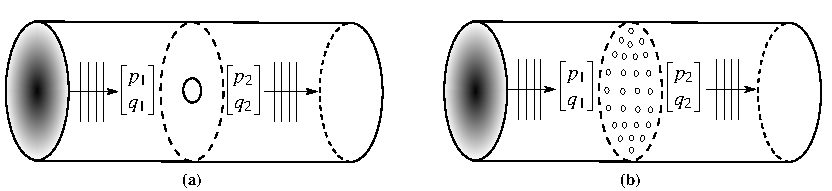
\includegraphics[scale=1]{images/0-/spp_mpp.pdf}
	\caption{Schematic representation of a propagating plane wave passing through a single (3a) and multiple (3b) perforate plate in the middle of a duct element and their respectively nodal pressure and volume velocity input and output vectors. Figure created by the author.}
	\label{fig:z_transf_scheme}
\end{figure}

The transfer matrix of a perforated element can be modeled as a transfer impedance series element in a two-port acoustic element system \cite{xin_thesis}. The \acrshort{MM} of a \acrfull{PP} (\acrfull{SPP} or \acrfull{MPP}) is as follows

\begin{equation} \label{eq:ztr_mm}
	\begin{bmatrix}
		-\frac{ S_p }{z_{tr}} & \frac{ S_p }{z_{tr}} \\
		\frac{ S_p }{z_{tr}} & -\frac{ S_p }{z_{tr}}\\
	\end{bmatrix}
	\begin{Bmatrix}
		p_1 \\
		p_2 \\
	\end{Bmatrix}
	=
	\begin{Bmatrix}
		q_1 \\
		q_2 \\
	\end{Bmatrix},
\end{equation}

\noindent where $S_p$ is the element cross-section area and the condition $q_1=q_2=u_n S_{\text{pp}}$ is considered.

In Fig.~\ref{fig:z_transf_scheme}, the scheme representation of \acrfull{SPP} and \acrfull{MPP} refers to an orientation of the \acrshort{PP} perpendicular to the main flow direction. In this case, when the flow pass through the holes of the \acrshort{PP} it is named as pure bias flow. The associated bias Mach number is generally denoted as $M_{\text{B}}$. 

The Fig.~\ref{fig:liner_2d} illustrates a \acrshort{PP}, also referred as liner, with an orientation parallel to the main flow direction (grazing flow). In this case, the holes of the \acrshort{PP} experiment bias flow as well as grazing flow. The associated grazing Mach number is generally denoted as $M_{\text{G}}$ representing the tangential flow in the \acrshort{PP} surface. The bias flow preserves the same concept as in Fig.~\ref{fig:z_transf_scheme}.

\begin{figure}[h!]
	\centering
	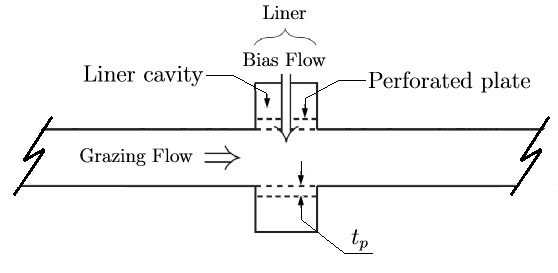
\includegraphics[scale=0.65]{images/0-/liner2D_grazing_biasflow.png} 
	\caption{A liner inside a cylindrical uniform duct under grazing and bias flow. Figure created by the author.}
	\label{fig:liner_2d}
\end{figure}

\subsection{Perforated plates impedance model}

A harmonic pressure and velocity variation is assumed, as in the \acrshort{LRF} fluid equivalent model presented in Subsection~\ref{subsubsec:lrf_damp}, to estimate the perforated plate impedance along the normal axis of a single cylindrical hole. Thus, it is possible to define the orifice impedance, $z_{orifice}$, as

\begin{equation} \label{eq:zorifice}
	z_{orifice} = \frac{\Delta p}{u_{\text{h}}} = \frac{p(x=0) - p(x=t_p)}{u(x=t_p/2)} = -2 i z_c \sin(k_c t_p' / 2),
\end{equation}

\noindent where $\Delta p$ is the pressure drop across the orifice, $u_{\text{h}}$ is the hole particle velocity, $t_p$ is the geometric plate thickness, $t_p'$ is the corrected plate thickness and $z_c$ and $k_c$ are the \acrshort{LRF} complex impedance and wavenumber, respectively, as were defined in Eqs.~\ref{eq:zc_lrfef}~and~\ref{eq:complex_wavenumber_lrf_ef}. The \acrshort{PP} geometrical parameters and related formulation variables are graphically shown in Fig.~\ref{fig:pp}.

In Eq.~\ref{eq:zorifice}, $u(x=t_p/2) = u_h$ is related to the orifice particle velocity, $u_h$, at the half of the \acrshort{PP} thickness (remember that $u_1=u_2$ was assumed). Through mass conservation, the duct particle velocity $u_1$ can be related to the hole particle velocity $u_h$ as \cite{Lee2005AcousticCO}

\begin{equation} \label{eq:mass_cons_pp}
	u_1 = \frac{n_h S_h}{S_1} u_h = \Phi u_h,
\end{equation}

\noindent where $n_h$ is the number of holes, $S_h$ is the area of a hole, $S_1$ is the duct area and $\Phi = (n_h S_h)/S_1 $ is the porosity. 

\noindent The linear specific impedance of a plate of diameter $d_{\text{pp}} = 2 r_i = d_i$ can be defined as

\begin{equation} \label{eq:zpp_linear_u1}
	z_{\text{pp,linear}} = \frac{p(x=0) - p(x=t_p)}{u_1}.
\end{equation}

\noindent The Eqs.~\ref{eq:zorifice}~to~\ref{eq:zpp_linear_u1} yield the relationship between the linear specific transfer impedance of a hole and a \acrshort{PP} as

\begin{equation} \label{eq:zpp_linear}
	z_{\text{pp,linear}} = \frac{z_{\text{orifice}}}{\Phi},
\end{equation}

\noindent where Eq.~\ref{eq:zpp_linear} is exact for ideal flow assumption, i.e., where the streamlines of the inviscid fluid flow through the hole are parallel to the longitudinal axis of the orifice (in Eqs.~\ref{eq:zorifice}~and~\ref{eq:zpp_linear_u1}, the $x$ axis). Specifically, the flow inside the orifice (and when it leaves the orifice) does not has radial velocity component. In practice, the ideal flow condition does not occur, i.e., viscothermal effect is important and the flow has a radial component velocity from the orifice upstream end to the downtream end, and also when it leaves the orifice \cite{MELLING19731}. This flow non-ideality is generally taken into account dividing Eq.~\ref{eq:zpp_linear} by a discharge coefficient, $C_{d,linear}$. Therefore, Eq.~\ref{eq:zpp_linear} becomes

\begin{equation} \label{eq:zpp_linear_nonideal}
	z_{\text{pp,linear}} = \frac{z_{\text{orifice}}}{\Phi C_{\text{d,linear}}},
\end{equation}

\noindent  where $C_{\text{d,linear}}$ is the linear discharge coefficient. In general, just one discharge coefficient is mentioned in the literature, named $C_{\text{d}}$, which conceptually, is a measure of how far the actual acoustic flow is from the ideal flow condition. However, for flexibility, there is a distinction between a linear and a non-linear discharge coefficient in \textit{OpenPulse}, depending on which impedance is being modeled (linear or non-linear). In \textit{OpenPulse}, the $C_\text{linear}$ parameter is defined by default with a unitary frequency independent value. For typical $C_d$ values and theoretical details the reader is invited to consult \cite{ MELLING19731,sun_pp,elnady_2003,zhou_pp}.

\subsection{\acrshort{ALC} of Perforated Plates} \label{subsec:alc_pp_chap3}

In  Eq.~\ref{eq:zorifice}, the corrected plate thickness $t_p'$ accounts for the effect of single and multiple holes in a partition of thickness $t_p$ across a tube of diameter $d_i$. This can be defined as

\begin{equation} \label{eq:pp_corrected_thickness}
	t_p' = t_p + 2\delta_{\text{lc,h}}',
\end{equation}

\noindent where $\delta_{\text{lc,h}}' = \delta_{\text{lc,h}} \Psi(\Phi) $ is the modified \acrshort{ALC} taking into account the hole~-~hole interaction and the effect of considering a finite partition of diameter $d_{\text{pp}} = d_i$, i.e. the presence of duct walls, through $\Psi(\Phi)$.

In \textit{OpenPulse}, the \acrshort{ALC} for a \acrshort{PP} is considered as a frequency independent parameter due to the fact that, for the plane wave assumption and for $He << 1$, the frequency dependence is small as for low $M$ values. In \textit{OpenPulse}, the \acrshort{ALC} of a \acrshort{PP} is calculated through the original formulation proposed by Fok \cite{fok,rschevkin}. Then, the modified \acrshort{ALC} $\delta_{\text{lc,h}}' = \delta_{\text{lc,h,Fok}}'$ is defined as 

\begin{equation} \label{eq:orifice_lengthcorr_fok}
	\delta_{lc,h,Fok}' = \frac{\pi r_h}{4} \Psi(\Phi),
\end{equation}

\noindent where $\Psi(\Phi)$ is the function of Fok defined as

\begin{equation} \label{eq:fok_sigma}
	\Psi (\Phi) = \sum_{i=0}^{12} a_i ( \Phi ) ^{i} ,
\end{equation}

\noindent where $a_0=$1, $a_1=$-1.4095, $a_2=$0, $a_3=$0.33818, $a_4=$0, $a_5=$0.0673, $a_6=-0.02287$, $a_7=$0.03015, $a_8=$-0.01641, $a_9=$0.01729, $a_{10}=$-0.01248, $a_{11}=$0.01205 and $a_{12}=$-0.00985, the twelve Fok's coefficients \cite{rschevkin}. In Eq.~\ref{eq:orifice_lengthcorr_fok}, $\pi r_h/4 = \delta_{lc,h}$ is equal to the \acrshort{ALC} lower limit for a cylindrical channel in an infinite plate deduced by Rayleigh in \cite{rayleigh1929theory}. The \texttt{Single hole} bottom in the \texttt{Add Perforated Plate} setup in \textit{OpenPulse} disables the effect of the Fok's function (it is replaced by a unitary constant value).

\subsection{Perforated plate nonlinear resistance} \label{subsec:pp_nonlinear}

When the fluid particle displacement becomes comparable to the diameter of the orifice, the vortex shedding can be described in terms of the formation of a free jet involving dissipation losses. These losses are due to the fact that the kinetic energy in the jet is dissipated by turbulence \cite{elnady_2003}. A good measure of vortices formation is the dimensionless parameter known as the acoustic Strouhal number, $Sr_{\text{ac}}$, which is given by

\begin{equation}
	Sr_{\text{ac}} = \frac{\omega r_{\text{h}}}{|u_{\text{h}}|} = \frac{He}{M_{\text{h}}},
\end{equation}

\noindent where $M_{\text{h}}$ is the hole Mach number defined as $M_{\text{h}} = |u_{\text{h}}|/c_f$ in which $|u_{\text{h}}|$ is the acoustic velocity amplitude at the PP hole. The variation of $Sr_{\text{ac}}$ characterizes different acoustic regimes, generally known as: strongly non-linear regime ($Sr_{\text{ac}} << 1$), transition regime ($Sr_{\text{ac}} = \mathcal{O}(1)$), almost linear regime (
$Sr_{\text{ac}} > 1$) \cite{TEMIZ} and linear regime ($Sr_{\text{ac}} >> 1$). Here a distinction is made between the acoustic Strouhal number ($Sr_{\text{ac}}$) and the Strouhal number ($Sr$). The latter is defined as $Sr = \omega r_{\text{h}} / M$ in which $M$ is the Mach number of the flow.

Generally, an additional term is added to the real part of the \acrshort{PP} impedance, $z_{\text{pp, linear}}$, to account for non-linear effects. $z_{\text{pp, linear}}$ depends on the acoustic particle velocity in the orifice and, indirectly, on the incident pressure ($p_1$). This term is named non-linear resistance, which is here named as $\theta_{\text{pp, linear}}$ in its dimensionless form. Naturally, the non-linear impedance also has an imaginary part named $\mathcal{I}(z_{\text{nl}})$. However, its influence is small for thin plates when compared with the loss of the end effects. 

Different expressions can be found in the literature for the non-linear resistance \cite{guess_1975, MELLING19731,elnady_2003, TEMIZ,zinn_1970}. However, the non-linear resistance term found in those formulations may be considered similar in the sense that the resistance expression term is proportional to the particle velocity. A general expression for the non-linear resistance, $\theta_{\text{pp, linear}}$, can be written in the following form, 

\begin{equation} \label{eq:non-linear_resistance}
	\theta_{\text{nl}} = \frac{ \mathcal{R} (z_{\text{nl}}) }{  z_{\text{f}} }= \frac{(1 - \Phi^2) f_{\text{nl}}}{2 \, (\Phi C_{\text{d,nl}})^2 \, c_0 } |u_{\text{n}}|,
\end{equation}

\noindent where $f_{\text{nl}}$ is a \acrshort{DOF} of Eq.~\ref{eq:non-linear_resistance}, generally used to adjust theoretical models with experimental non-linear resistance data \cite{elnady_2003}. $C_{\text{d,nl}}$ is the nonlinear discharge coefficient which was distinguished from $C_{\text{d,linear}}$ with the aim of giving a more general non-linear resistance $\theta_{\text{nl}}$ definition, taken into account that $|u_{\text{n}}|$ is large enough; thus, $C_{\text{d,linear}} \neq C_{\text{d,non-linear}}$. The factor $(1 - \Phi^2) f_{\text{nl}} / (\Phi C_{\text{d,nl}})^2$ in Eq.~\ref{eq:non-linear_resistance} results from the non-ideal flow \cite{MELLING19731} and depends on the certainty on the parameters $C_{\text{d,nl}}$ and $f_{\text{nl}}$. Both of them may be dependent on frequency, pressure, medium velocity and hole geometry. In \textit{OpenPulse} the $C_{\text{d,nl}}$ and $f_{\text{nl}}$ parameters are defined with the frequency independent default values 0.76 and 1, respectively. For detailed information about these specific parameters, the reader is invited to consult \cite{elnady_2003,elnady_thesis,discharge_zhou,TEMIZ}.

In Eq.~\ref{eq:non-linear_resistance}, $u_n$ is the acoustic particle velocity magnitude normal to the \acrshort{PP} surface, which can be determined from the \acrshort{PP} impedance definition

\begin{equation} \label{eq:un-iterative}
	| u_{\text{n}} | = \Big| \frac{ p_{\text{pp}} }{z_{\text{pp}}} \Big|,
\end{equation}

\noindent where $p_{pp}$ is the \acrshort{PP} surface acoustic pressure and $z_{pp}$ the \acrshort{PP} specific impedance. However, it is not possible to directly calculate $\theta_{nl}$ because the non-linear resistance now depends on $|u_n|$, and the $u_n$ value is not known without solving first the global acoustic system including the \acrshort{PP}. To solve this issue, an iterative process of Eq.~\ref{eq:un-iterative} is proposed in order to achieve a $|u_n|$ value. Therefore, the computation of the $|u_n|$ value will depend on the availability of the pressure amplitude value close to the \acrshort{PP} surface.  In \textit{OpenPulse}, a relation between the pressure amplitude close to the \acrshort{PP} surface and normal velocity of the \acrshort{PP} is proposed. Then, the \acrshort{PP} $u_n$ values are obtained using the perforated plate upstream and downstream nodal acoustic pressure amplitude values. This idea is expressed through the \acrshort{PP} normal velocity definition based on the transfer impedance of Eq.~\ref{eq:ztr}

\begin{equation} \label{eq:un-up-down}
	| u_n | = \Big| \frac{(p_{\text{upstream}}-p_{\text{downstream}})}{z_{\text{pp}}} \Big|.
\end{equation}

\subsection{\acrshort{PP} radiation resistance}

The resistive part of the radiation impedance accounts for the acoustic losses by radiation into the surrounding medium \cite{LAHIRI2017564}. An expression for the mechanical impedance of the radiation load on a piston face (i.e., flanged open-ended tube), due to radiation effects, is derived by Morse and Ingard \cite{morse1986theoretical}. Therefore, the dimensionless radiation impedance of a \acrshort{PP} with porosity $\Phi$ and holes of diameter $d_h$ is \cite{morse1986theoretical}:

\begin{equation} \label{eq:radiation_imp_ingard}
	\xi_{rad} = z_{rad}/ z_{\text{f}} =  \frac{1}{\Phi} \Big( \Big[ 1 - \frac{J_1(2 He_h)}{He_h} \Big] - i \frac{4}{\pi} \int_{0}^{\pi/2} \sin(2He_h \cos(\Omega)) \sin(\Omega)^2 \text{d}\Omega \Big),
\end{equation}

\noindent where $He_h = k r_h$ is the hole Helmholtz number and $\Omega$ is the integration variable. To represent the radiation resistance, only the real part of Eq.~\ref{eq:radiation_imp_ingard} is implemented in \textit{OpenPulse}. Then,

\begin{equation} \label{eq:radiation_imp}
 	\theta_{rad} = z_{rad}/ z_{\text{f}} =  \frac{1}{\Phi} \Big(  1 - \frac{J_1(2 He_h)}{He_h} \Big).
\end{equation}

\subsection{\acrshort{PP} bias flow resistance}

In the case that the \acrshort{PP} has a disposition perpendicular to the steady mean flow, as indicated in Fig.~\ref{fig:z_transf_scheme}, the mean flow effects are taken into account considering a unique pure bias flow resistance as follows 

\begin{equation} \label{eq:induct_pp_bias_flow}
	\theta_B = \mathfrak{R}(z_{B})/ z_{\text{f}} = k_\text{B} \frac{(1 - \Phi^2) }{ \Phi C_d^2  } M,
\end{equation}

\noindent where $k_\text{B}$ is the bias flow coefficient, a \acrshort{DOF} parameter useful to control the contribution of the acoustic resistance due to mean flow. In addition, the \acrshort{PP} impedance can be fitted with experimental data results if available. In \textit{OpenPulse}, $k_\text{B}$ has a unitary frequency independent default value.

A similar approach to Eq.~\ref{eq:induct_pp_bias_flow} was proposed by Cummings and Eversman \cite{CUMMINGS1983503} for high amplitude pressure waves. Cummings and Eversman \cite{CUMMINGS1983503} mention that when 2$M >> |u_n/c_0|$ the non-linear contribution of Eq.~\ref{eq:induct_pp_bias_flow} to the \acrshort{PP} impedance $z_{\text{pp}}$ will be swamped by the mean flow dependent term.  

%In the experimental results obtained in the work of Spillere et al. \cite{spillere2016_pp}, the grazing $M$ dependent terms (Eqs.\ref{eq:grazing_flow}~and, probably~\ref{eq:induct_pp_bias_flow} ) dominate in the contribution to the liner resistance, as expected and aforementioned. In addition, a frequency dependency is observed when the real part of several literature liner impedance models are compared with the liner resistance experimental data in \cite{spillere2016_pp}. 

\subsection{Final PP impedance and FETM implementation}

In Eqs.~\ref{eq:zorifice}~,~\ref{eq:zpp_linear_u1}~,~\ref{eq:zpp_linear}~and~\ref{eq:zpp_linear_nonideal}, the \acrshort{PP} impedance  $z_{\text{pp}}$ is negative defined. In the final \acrshort{PP} impedance computation, any term to be added to the basic $z_{\text{pp,linear}}$ expression of Eq.~\ref{eq:zpp_linear_nonideal} needs to be calculated as follows

\begin{equation} \label{eq:zpp_final}
	z_{pp} = z_{\text{pp,linear}} -  z_{\text{f}} ( \theta_{nl} + \xi_{\text{rad}} + \theta_B ),
\end{equation}

\noindent for a \acrshort{PP} disposition as in Fig.~\ref{fig:z_transf_scheme} and where Eqs.~\ref{eq:zpp_linear_nonideal}~,~\ref{eq:non-linear_resistance}~,~\ref{eq:un-up-down}~,~\ref{eq:radiation_imp}~and~\ref{eq:induct_pp_bias_flow} are the indicated equations for the computation of $z_{pp}$ in this case. 

%where $z_{pp,linear}$ was negative defined in Eqs.~\ref{eq:zorifice}~and~\ref{eq:zpp_linear} and $\theta_{nl}$ was (negative) added to the final expression of $z_{pp}$. 
%
%Other impedances can be (negative) added to account for a better representation of the physical phenomena that occur in a PP (e.g. radiation impedance and bias and/or grazing flow effects). As an starting point the reader can consult the cited bibliography along this section.

The main goal of this section is to present the implementation of Eq.~\ref{eq:zpp_final} using the \acrshort{MM} of Eq.~\ref{eq:ztr_mm}. The following computational scheme can be followed to iteratively calculate a \acrshort{GMM} system including a \acrshort{PP} accounting for non-linear effects (Eq.~\ref{eq:zpp_final}), as well as other \acrshort{BC's} forming the global \acrshort{MM}.

\begin{enumerate}
	\item Calculate Eq.~\ref{eq:zpp_final} without non-linear effect term, i.e. $u_n= 0 $ m/s.
	\item Solve the \acrshort{GMM} system. Save $p_{upstream}$ and $p_{downstream}$ for each frequency step.
	\item Calculate Eq.~\ref{eq:un-up-down}.
	\item Calculate Eq.~\ref{eq:zpp_final} with non-linear effect term, i.e. using $|u_n|$ from step 3.
	\item Calculate the criteria stop for each $N$-iteration as
	\begin{equation} \label{eq:convergence_pp}
		\frac{|| p_{N , upstream}  -  p_{N-1,upstream} ||_2}{ || p_{N,upstream}||_2}  < tolerance = 0.01.
	\end{equation}
	% with $p_{n-1,avrg}$ defined as
	% \begin{equation}
		%     p_{n-1,avrg} = \frac{ p_{n-1 , upstream} + p_{n-1,upstream}}{2}.
		% \end{equation}
	\item If $tolerance$ is achieved in step 5, stop. If not, return step 3.
	%	\item Repeat steps 3-6 $N$-times.
\end{enumerate}

\subsection{Meelling's \acrshort{PP} impedance model}

The \acrshort{PP} impedance model of Melling \cite{MELLING19731} is implemented in \textit{OpenPulse} as a way to compare the previously presented \textit{OpenPulse's} \acrshort{PP} impedance model. The impedance model of Melling is a reference literature model and was largely tested in several works with impedance experimental data. However, this model only applies for a stagnant fluid medium. In \textit{OpenPulse}, the formulation available in the work of Melling \cite{MELLING19731} is implemented as

 
\begin{equation}
	\xi_{Melling} = z_{Melling}/ z_f = \frac{ik_0}{\Phi C_d} \bigg( \frac{t_p}{F(k_s' r_h)} + \frac{16 r_h / (3\pi)  }{F(k_s r_h)} \Psi'(\sqrt{\Phi})\bigg) + \frac{4 (1-\Phi^2)}{ 3 \pi c_0 \, ( \Phi C_d)^2 } |u_n|,
\end{equation}

\noindent where the function $F$ introduces the viscous effects as $F(x) = 1 - \frac{2J_1(x)}{x J_0(x)}$, $k_s = \sqrt{-i\omega / \nu}$ is the Stoke's wavenumber (considering only viscocity effect)), $k_s' = \sqrt{-i\omega / \nu'}$ is the effective Stokes wavenumber (considering thermal and viscocity effects) through an effective kinematic fluid viscocity $\nu' = 2,179 \nu$ and $z_f=\rho_f c_f$ the characteristic impedance of the medium.

\subsection{\texttt{Common pipe section}}

The \texttt{Common pipe section} option is the third possibility in \texttt{OpenPulse} to model a flow constriction in a gas pipeline system. When this option is enable, only the hole diameter can be edited in the \textit{OpenPulse} \acrshort{PP} plate setup. The \texttt{acoustic element type} will automatically be adopted as the same type of the acoustic elements located at each side of the constriction. Then, the constriction is modeled as a duct element, i.e., using the \acrshort{MMs} of Eqs.~\ref{eq:mmm_element_expand}~and~\ref{eq:MM_flow-acoustic} and related damping models.

\section{\texttt{Set Element Length Correction}}

As the AIV phenomena has 3D complexity in nature, 1D \acrshort{TM} elements have been developed over 40 years to get a simple and accurate description of \acrshort{AIV} transmission in gas piping systems. However, there are certain limitations in the application of 1D-\acrshort{TMM} plane wave element. These limitations can be generally related to proper aspects of 1D formulation (frequency range), geometry shape or certain geometry aspect relations of the acoustic geometry) and related methods (as \acrshort{TMM}, \acrshort{MMM} and \acrshort{FETM}).

In the \acrshort{TMM} or \acrshort{FETM}, the \acrfull{GMM} is formed by assembling the elements (\acrshort{TM} or \acrshort{MM}) together, using the fact that at the coupling nodes the acoustic pressures are equal  and the sum of the volume source terms must be zero \cite{craggs1990, acoustics1d, FRID1989423}. However, in two-port networks under low-frequency assumption, wave propagation in coupled elements could be not accurately described in the transition zones between elements (as is the case of a cross junction, a T-junction (side branches) and a sudden expansion or contraction) under certain conditions.

With the application of an \acrfull{ALC} in a 1D model, the higher order modes of a wave propagation are artificially included through an additive extension of the waveguide element length. This additive length correction needs to be applied in the waveguide element with the smallest cross-sectional dimension \cite{nijhofthesis2010, mareze_jsv} as indicated in Fig.~\ref{fig:lc_scheme} for classical geometry junction discontinuities commonly found in gas pipeline systems.  When an \acrshort{ALC} is applied at geometry junctions as side branches, loops and sudden expansions or contractions, the local effects prediction capability is improved, tending to a better representation of the field
for both pressure and velocity.

%\begin{figure}[h]
%	\centering
%	\includegraphics[scale=0.55]{images/3-/lc_sb_sce.png}
%	\caption{ \acrshort{ALC} application in side branche and sudden contraction/expansion geometries.}
%	\label{fig:lc_sb_sce}
%\end{figure}

\begin{figure}[ht!]
	\centering
	\begin{subfigure}[b]{0.3\textwidth}
		\centering
		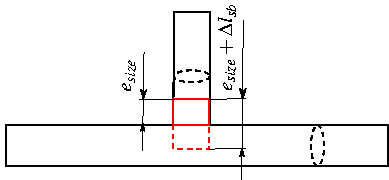
\includegraphics[scale=0.85]{images/0-/lc_sb.pdf}
		\caption{}
		\label{fig:lc_sb_scheme}
	\end{subfigure}
	\hspace{-1mm}
	%\hfill
	\begin{subfigure}[b]{0.3\textwidth}
		\centering
		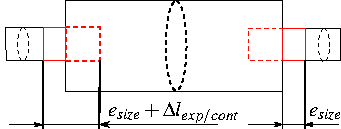
\includegraphics[scale=1]{images/0-/lc_exp.pdf}
		\caption{}
		\label{fig:lc_exp_scheme}
	\end{subfigure}
	\hspace{5mm}
	%\hfill
	\begin{subfigure}[b]{0.3\textwidth}
		\centering
		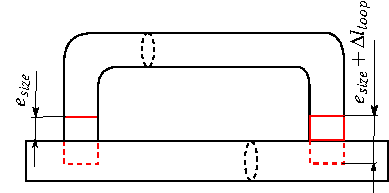
\includegraphics[scale=0.875]{images/0-/lc_loop.pdf}
		\caption{}
		\label{fig:lc_loop_scheme}
	\end{subfigure}
	\caption{\acrshort{ALC} implementation scheme for \ref{fig:lc_sb_scheme} side branch, \ref{fig:lc_exp_scheme} sudden expansion/contraction and \ref{fig:lc_loop_scheme} loop geometries. Figure created by the author.}
	%	\label{fig:lc_all}
	\label{fig:lc_scheme}
\end{figure}

It is important to note that, in \textit{OpenPulse}, the term \acrshort{ALC} is called when a waveguide element length correction is applied in a quiescent fluid background condition ($M=$0). When a moving medium fluid background condition ($M>$0) is being considered inside a waveguide, the term \acrfull{FALC} is used. In a more general way, both the \acrshort{ALC} and the \acrshort{FALC} terms are considered as \acrfull{WLC}.

\subsection{Expansion}

Sudden expansion/contraction geometry types are frequently found in pipeline systems, e.g., as part of expansion chambers (Fig.~\ref{fig:lc_exp_scheme}). One of the first in modeling the \acrshort{ALC} of a sudden area expansion or contraction was Karal \cite{karal}. The resultant model formulation is based on an impedance model of a sudden area change in a cylindrical waveguide considering undamped wave propagation. As a result, the effect of the discontinuity is reflected as the introduction of an inductance in series with the acoustic waveguide (upstream of the expansion or contraction) named ``constriction inductance''. This impedance can be considered as a correction term that is added to the analogous acoustical inductance of a tube of circular cross-section. Physically, it may be interpreted as an increase in the physical length of the tube ($\Delta l_{\text{exp/cont}}$). The \acrshort{ALC} of a cylindrical sudden area change proposed by Karal \cite{karal} is reproduced as
%
\begin{gather} \label{eq:lc_exp}
	\Delta l_{\text{exp/cont}} = \frac{8 r_{i,minor} }{ 3 \pi} H( \xi_{\text{r,exp/cont}} ) , \\ \label{eq:lc_exp_b}
	H( \xi_{\text{r,exp/cont}} ) = \frac{3 \pi }{ 2}  \sum_{m=1}^{\infty} \frac{J_1^2( j_m \xi_{\text{r,exp/cont}} )}{ j_m \xi_{\text{r,exp/cont}}  ( j_m J_0(j_m))^2 },
\end{gather}

\noindent where $H( \xi_{\text{r,exp/cont}} )$ is the discontinuity inductance correction factor (also known as Karal's factor), $\xi_{\text{r,exp/cont}} = r_{\text{i,minor}}/r_{\text{i,major}}$ is the ratio of radii between the minor and major duct radii present at the discontinuity (i.e, sudden expansion or contraction), and $j_m$ is the mth-root of the equation $J_1(j_m)=0$. 

The implementation of Eq.~\ref{eq:lc_exp_b} depends on the considered quantity of summation terms and on first kind Bessel functions. This may result in a high computational cost or in problems with the order of the argument in the Bessel functions (small or big argument). Consequently, a helpful polynomial expression given in \cite{daSilva_nunes} for Eq.~\ref{eq:lc_exp_dasilva} is implemented in \textit{OpenPulse} and reproduced here as

\begin{equation} \label{eq:lc_exp_dasilva}
	\Delta l_{\text{exp/cont}} = 
	\begin{cases}
		\frac{8 r_{\text{i,minor}} }{ 3 \pi} (1 - 1.238 \xi_{\text{r,exp/cont}}  ), \hspace{10mm} & \xi_{\text{r,exp/cont}}  \leq 0.5, \\
		\frac{8 r_{\text{i,minor}} }{ 3 \pi} \big( 0.875 (1 - \xi_{\text{r,exp/cont}}  )(1.371 - \xi_{\text{r,exp/cont}}  ) \big),  &  \xi_{\text{r,exp/cont}}  > 0.5.
	\end{cases}
\end{equation}

Eq.~\ref{eq:lc_exp} is clearly frequency independent ($He \rightarrow$0 solution) and is developed considering an undamped wave propagation. However, Karal \cite{karal} derived $H(\xi_{\text{r,exp/cont}})$ in Eq.~\ref{eq:lc_exp} replacing the frequency dependent terms in all expressions by constants. This approximation is only valid in the low frequency limit ($He \rightarrow$0) and gives a discontinuity inertance $H$ that
only depends on the radius ratio parameter $\xi_{\text{r,exp/cont}}$, i.e, $H( \xi_{\text{r,exp/cont}} )$ \cite{peat_exp_falc}. 

\subsection{Side branch}

Side branches are commonly found in industry gas pipeline systems. As shown in Fig.~\ref{fig:lc_sb_scheme}, side branches usually have an open (lower) and a closed or rigid (upper) end. The denomination ``open end \acrshort{ALC}'', frequently found in the literature \cite{dang}, refers when the \acrshort{ALC} is applied in the open end of the side branch. In the case of an upper rigid or closed extreme, the side branch is often called ``dead leg''. However, there are also in industry side branches that are modeled with an anechoic impedance termination, indicating that the pipeline end is far away from the junction point. 

In literature it is often found open end \acrshort{ALC} for side branches modeled with rigid end and undamped wave propagation as in the work of Ji \cite{JI}, in which a \acrshort{BEM} approach was used to solve a 3D cylindrical side branch placed at a main duct. To avoid (local) finite waveguide effect, the lengths of the side branch and each main duct section need to be at least twice their diameters \cite{JI}. Also, if $He<$0.5, the \acrshort{ALC} frequency dependence can be neglected \cite{dalmont_sb, JI}, the plane wave condition is ensured, and the following low-frequency \acrshort{ALC} approximation ($He \rightarrow 0$) for side branches with rigid end proposed by Ji \cite{JI} is reproduced as

\begin{equation} \label{eq:lc_sb_ji}
	\Delta l_{\text{sb}} = 
	\begin{cases}
		r_{i,sb} \big( 0.8216 - 0.0644  \xi_{\text{r,sb}}  - 0.694  \xi_{\text{r,sb}} ^2 \big), \hspace{10mm} & \xi_{\text{r,sb}} \leq 0.4, \\
		r_{i,sb} \big( 0.9326 -0.6196 \, \xi_{\text{r,sb}} \big),  &  \xi_{\text{r,sb}} > 0.4,
	\end{cases}
\end{equation}

\noindent where $\xi_{\text{r,sb}}= r_{i,sb}/ r_{i, duct}$ is the ratio between the side branch and main duct radii at the side branch discontinuity type. Eq.~\ref{eq:lc_sb_ji}  is implemented in \textit{OpenPulse}.

\subsection{Loop}

Loop type geometries, or pipes arranged in a parallel configuration (like a by-pass), are frequently found in natural gas pipeline systems (Fig.~\ref{fig:lc_loop_scheme}). To the author knowledge, there are not \acrshort{ALC} formulations for loop geometry types in the literature. In \textit{OpenPulse}, trough numerical experiments and comparisons with 3D \acrshort{FEM} results, it was determined that computing \acrshort{ALC} for loop discontinuities with Eq.~\ref{eq:lc_exp} gives better results in both frequency shift and magnitude response than if using Eq.~\ref{eq:lc_sb_ji}. This is probably explained by the fact that for side branches the \acrshort{ALC} formulation is developed with rigid end \acrshort{BC}. This \acrshort{BC} is not representative for the loop type geometry in which a continuity of pressure and volume velocity exists between the loop beginning and end \cite[see Fig.~2 and Eqs.~12~to~24 in][]{TO_1}. Another explanation may be associated with the loop length and the assumptions made in the \acrshort{ALC} formulation related with Eq.~\ref{eq:lc_sb_ji}. If the loop length is not sufficiently long, evanescence waves effects at the loop-main duct junction cannot be neglected.

\subsection{\acrshort{WLC} in a moving medium} 

In the case of considering a plane wave propagation in a moving fluid medium ($M > 0$), the corresponding 1D elements length can also be corrected. In this case, a \acrshort{FALC} can be applied in the junction of the same geometries than for the \acrshort{ALC} case. Briefly, a general behavior for the \acrshort{FALC} can be described, since for low $M$ exists, in general, a region in which there is not interaction between the acoustic wave and the moving fluid medium, i.e., the \acrshort{FALC} remains constant. When $M$ increases, at a certain value (geometry dependent), the \acrshort{FALC} value starts to decrease up to a point in which its value is null, i.e., the effective waveguide element length equals the geometrical waveguide element length and no length correction is needed. The decrease in the \acrshort{FALC} value means that mean flow effects totally dominate over the acoustic wave propagation.

Currently in \textit{OpenPulse}, there are not implement any \acrshort{FALC} formulation. In the region where there are no interaction between the acoustic wave and the moving fluid medium, the implemented \acrshort{ALC}s can be carefully used. However, it is being assumed that at low $M$ values and for the presented geometry junction types, exist a no interaction region between the acoustic wave and the moving fluid medium.

\section{\texttt{Add Compressor Excitation}}

The compressor excitation is another volume velocity \acrshort{BC} (Section~\ref{sec:bc_vol_vel}). It represents a simplified reciprocating compressor model which gives the acoustic volume velocity values as a function of frequency at the suction or discharge points in a typical reciprocating compressor. The theory for modeling the compressor excitation can be found in, e.g., Chapter~5 in \cite[][]{fiv_kaneko} and in  Chapter~11 in \cite[][]{botros2018pipeline}. 

The simple model associated with just one side of the piston and neglecting the dynamics of the valve is based on the piston kinematics, which gives the source volume velocity at the piston face $q_\text{RC}$ as a function of time $t$ as follows \cite{botros2018pipeline}, 

\begin{equation} \label{eq:compressor_model}
q_\text{RC} = - S_\text{p} R \omega \sin(\theta) \Bigg[ 1 + \frac{R}{L} \frac{\cos(\theta)}{\sqrt{1 - \Big( \frac{R}{L} \sin(\theta) \Big)^2 }} \Bigg],
\end{equation}


\noindent where $S_\text{p}$ is the reciprocating piston effective area, $R$ is the crank radius, $L$ is the connecting rod length, $\omega$ is the crank angle from top dead center ($\theta = \omega t$) and $\omega$ is the rotational speed in $rad/s$. A complete setup related with parameters of the reciprocating compressor, typically found in an equipment technical sheet, and with the signal processing of Eq.~\ref{eq:compressor_model} (function varying in time) can be adjusted to obtain a desired compressor model.



%------------------------------------------------------------------
% 
%------------------------------------------------------------------
\newpage
% 
\bibliographystyle{plain}
\bibliography{references}
\end{document}
